\documentclass[14pt]{beamer}
\usepackage{./Estilos/BeamerUVM}
\usepackage{./Estilos/ColoresLatex}
%Sección para el tema de beamer, con el theme, usercolortheme y sección de footers
\usetheme{CambridgeUS}
\usecolortheme{default}
%\useoutertheme{default}
\setbeamercovered{invisible}
% or whatever (possibly just delete it)
\setbeamertemplate{section in toc}[sections numbered]
\setbeamertemplate{subsection in toc}[subsections numbered]
\setbeamertemplate{subsection in toc}{\leavevmode\leftskip=3.2em\rlap{\hskip-2em\inserttocsectionnumber.\inserttocsubsectionnumber}\inserttocsubsection\par}
\setbeamercolor{section in toc}{fg=blue}
\setbeamercolor{subsection in toc}{fg=blue}
\setbeamercolor{frametitle}{fg=blue}
\setbeamertemplate{caption}[numbered]

\setbeamertemplate{footline}
\beamertemplatenavigationsymbolsempty
\setbeamertemplate{headline}{}


\makeatletter
\setbeamercolor{secºtion in foot}{bg=gray!30, fg=black!90!orange}
\setbeamercolor{subsection in foot}{bg=blue!30!yellow, fg=red}
\setbeamercolor{date in foot}{bg=black, fg=white}
\setbeamertemplate{footline}
{
  \leavevmode%
  \hbox{%
  \begin{beamercolorbox}[wd=.333333\paperwidth,ht=2.25ex,dp=1ex,center]{section in foot}%
    \usebeamerfont{section in foot} \insertsection
  \end{beamercolorbox}%
  \begin{beamercolorbox}[wd=.333333\paperwidth,ht=2.25ex,dp=1ex,center]{subsection in foot}%
    \usebeamerfont{subsection in foot}  \insertsubsection
  \end{beamercolorbox}%
  \begin{beamercolorbox}[wd=.333333\paperwidth,ht=2.25ex,dp=1ex,right]{date in head/foot}%
    \usebeamerfont{date in head/foot} \insertshortdate{} \hspace*{2em}
    \insertframenumber{} / \inserttotalframenumber \hspace*{2ex} 
  \end{beamercolorbox}}%
  \vskip0pt%
}






% \usefonttheme{serif}
\usepackage[clock]{ifsym}
\usepackage{pstricks-add}
\DeclareSIUnit\erg{erg}
\DeclareSIUnit[number-unit-product = {\,}]\cal{cal}

\sisetup{per-mode=symbol}
\resetcounteronoverlays{saveenumi}

% Macro para agregar el logo de UVM en cada slide de la presentación

\addtobeamertemplate{frametitle}{}{%
\begin{tikzpicture}[remember picture,overlay]
\coordinate (logo) at ([xshift=-1.5cm,yshift=-0.8cm]current page.north east);
% \fill[devryblue] (logo) circle (.9cm);
% \clip (logo) circle (.75cm);
\node at (logo) {
\includegraphics[width=2.1cm]{Imagenes/logo_UVM.png}};
\end{tikzpicture}}


\title{\Large{Sustentabilidad y contaminación} \\ \normalsize{Física III}}
\date{}

\begin{document}
\maketitle

\section*{Contenido}
\frame[allowframebreaks]{\frametitle{Contenido} \tableofcontents[currentsection, hideallsubsections]}

\section{Sustentabilidad}
\frame{\tableofcontents[currentsection, hideothersubsections]}
\subsection{¿Qué es la sustentabilidad?}

\begin{frame}
\frametitle{Definición de sustentabilidad}
La \textocolor{red}{sustentabilidad} se refiere a la capacidad de \textocolor{cobalt}{satisfacer las necesidades presentes} \pause \textocolor{bole}{sin comprometer la capacidad de las futuras generaciones} para satisfacer sus propias necesidades.
\end{frame}
\begin{frame}
\frametitle{Definición de sustentabilidad}
La sustentabilidad implica equilibrar los aspectos económicos, sociales y ambientales para garantizar un desarrollo sostenible a largo plazo.
\end{frame}
\begin{frame}
\frametitle{Sustentabilidad}
\begin{figure}
    \centering
    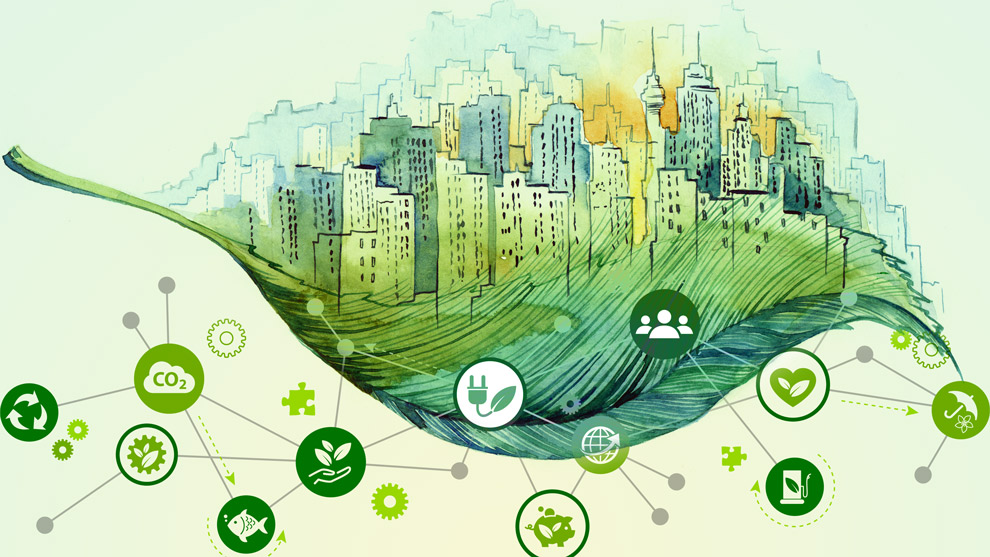
\includegraphics[scale=0.25]{Imagenes/Sustentabilidad_01.jpg}
\end{figure}
\end{frame}
\begin{frame}
\frametitle{¿Cómo lograr la sustentabilidad?}
Es importante reconocer que los elementos ambientales, económicos y sociales \textocolor{coquelicot}{están interconectados}.
\end{frame}
\begin{frame}
\frametitle{¿Cómo lograr la sustentabilidad?}
Los recursos \textocolor{ao(english)}{son finitos} y deben de usarse con objetivos a largo plazo.
\end{frame}

\section{Física y contaminación}
\frame{\tableofcontents[currentsection, hideothersubsections]}
\subsection{Intervención de la física}

\begin{frame}
\frametitle{La física y contaminación}
La física desempeña un papel importante en el \textocolor{americanrose}{estudio}, la \textocolor{auburn}{comprensión} y la \textocolor{brown(web)}{mitigación} de la contaminación en sus diversas formas.
\end{frame}
\begin{frame}
\frametitle{Dispersión de contaminantes}
La física proporciona \textocolor{cadmiumred}{modelos matemáticos} y \textocolor{carmine}{herramientas computacionales} para predecir cómo se dispersan los contaminantes en la atmósfera, el agua y el suelo.
\end{frame}
\begin{frame}
\frametitle{Dispersión de contaminantes}    
Estos modelos se basan en principios físicos como la \textocolor{carnelian}{difusión}, la \textocolor{cerise}{convección} y la \textocolor{cinnabar}{advección}.
\end{frame}
\begin{frame}
\frametitle{Dispersión de contaminantes}
Esos modelos ayudan a los científicos y los gestores del medio ambiente a comprender la dinámica de los contaminantes y a tomar medidas adecuadas para su control.
\end{frame}
\begin{frame}
\frametitle{Monitoreo de la contaminación}
La física ofrece una variedad de técnicas y dispositivos para \textocolor{cornellred}{medir la concentración} de contaminantes en el aire, el agua y el suelo.
\end{frame}
\begin{frame}
\frametitle{Monitoreo de la contaminación}
Esto incluye instrumentos como espectrómetros, sensores remotos, cromatógrafos y detectores de partículas. 
\end{frame}
\begin{frame}
\frametitle{Monitoreo de la contaminación}
Estos instrumentos permiten a los científicos y a las agencias ambientales realizar un seguimiento de la calidad del medio ambiente y evaluar el cumplimiento de los estándares de calidad del aire y del agua.
\end{frame}
\begin{frame}
\frametitle{Tratamiento de residuos}
La física también se utiliza en el diseño y la operación de tecnologías para el tratamiento de residuos y contaminantes.
\end{frame}
\begin{frame}
\frametitle{Tratamiento de residuos}
Esto incluye procesos como la filtración, la destilación, la oxidación, la adsorción y la fotocatálisis, que se basan en principios físicos para eliminar los contaminantes del aire y el agua.
\end{frame}
\begin{frame}
\frametitle{Energías renovables}
La contaminación del aire y del agua está estrechamente relacionada con la quema de combustibles fósiles y la generación de energía.
\end{frame}
\begin{frame}
\frametitle{Energías renovables}
La física desempeña un papel importante en el desarrollo y la implementación de tecnologías de energía renovable.
\end{frame}
\begin{frame}
\frametitle{Energías renovables}
Como la energía solar, eólica, hidroeléctrica y geotérmica, que tienen un menor impacto ambiental y contribuyen a reducir las emisiones de gases de efecto invernadero.
\end{frame}

\section{Efecto invernadero}
\frame{\tableofcontents[currentsection, hideothersubsections]}
\subsection{¿Qué es el efecto invernadero?}

\begin{frame}
\frametitle{El efecto invernadero}
El efecto invernadero es un \textocolor{ao(english)}{proceso natural} y esencial para mantener la temperatura de la Tierra en niveles adecuados para la vida.
\end{frame}
\begin{frame}
\frametitle{El efecto invernadero}
Este fenómeno ocurre cuando ciertos gases en la atmósfera terrestre, conocidos como \textocolor{ao}{gases de efecto invernadero (GEI)}, absorben y emiten radiación infrarroja.
\end{frame}
\begin{frame}
\frametitle{El efecto invernadero}
Lo que provoca que parte del calor emitido por la superficie terrestre sea \textocolor{red}{retenido y reenviado de vuelta a la superficie}.
\end{frame}
\begin{frame}
\frametitle{El efecto invernadero}
Esto crea un efecto similar al que se observa en un invernadero, \pause donde el vidrio permite que la luz solar entre pero impide que el calor se escape.
\end{frame}
\begin{frame}
% \frametitle{El efecto invernadero}
\vspace*{-0.5cm}
\begin{figure}
    \centering
    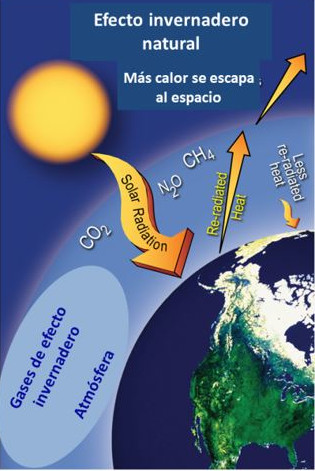
\includegraphics[scale=0.6]{Imagenes/Efecto_Invernadero_02.jpg}
\end{figure}
\end{frame}
\begin{frame}
% \frametitle{El efecto invernadero}
\vspace*{-0.5cm}
\begin{figure}
    \centering
    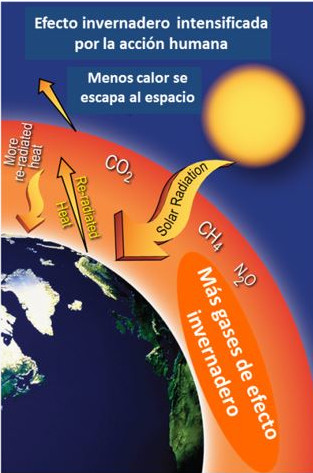
\includegraphics[scale=0.6]{Imagenes/Efecto_Invernadero_03.jpg}
\end{figure}
\end{frame}
 
\subsection{Gases de efecto invernadero}

\begin{frame}
\frametitle{Gases de efecto invernadero}
Los principales gases de efecto invernadero en la atmósfera incluyen:
\pause
\setbeamercolor{item projected}{bg=cobalt,fg=white}
\setbeamertemplate{enumerate items}{%
\usebeamercolor[bg]{item projected}%
\raisebox{1.5pt}{\colorbox{bg}{\color{fg}\footnotesize\insertenumlabel}}%
}
\begin{enumerate}[<+->]
\item Dióxido de carbono (CO2)
\item Metano (CH4)
\seti
\end{enumerate}
\end{frame}
\begin{frame}
\frametitle{Gases de efecto invernadero}
\setbeamercolor{item projected}{bg=cobalt,fg=white}
\setbeamertemplate{enumerate items}{%
\usebeamercolor[bg]{item projected}%
\raisebox{1.5pt}{\colorbox{bg}{\color{fg}\footnotesize\insertenumlabel}}%
}
\begin{enumerate}[<+->]
\conti
\item Óxidos de nitrógeno (NOx)
\item Ozono (O3)
\item Vapor de agua (H2O)
\end{enumerate}
\end{frame}
\begin{frame}
\frametitle{Gases de efecto invernadero}
Estos gases son liberados \textocolor{debianred}{naturalmente} por procesos biológicos y geológicos
\end{frame}
\begin{frame}
\frametitle{Gases de efecto invernadero}
Así como por actividades humanas como la quema de combustibles fósiles, la deforestación y la agricultura.
\end{frame}

\section{Inversión térmica}
\frame{\tableofcontents[currentsection, hideothersubsections]}
\subsection{¿Qué es la inversión térmica?}

\begin{frame}
\frametitle{Definición de la inv. térmica}
Por lo regular a nivel de piso la temperatura \textocolor{red}{es más caliente} \pause y las capas superiores \textocolor{ao}{son más templadas}, predominando posteriormente aire frío.
\end{frame}
\begin{frame}
% \frametitle{Inversión térmica}
\begin{figure}
    \centering
    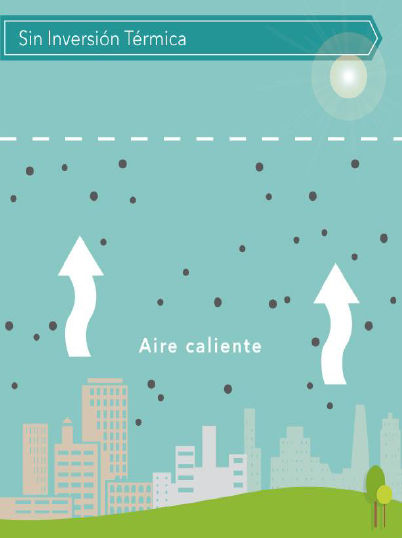
\includegraphics[scale=0.5]{Imagenes/Inversion_Termica_01.png}
\end{figure}
\end{frame}
\begin{frame}
\frametitle{Definición de la inv. térmica}
Cuando sucede el fenómeno de la inversión térmica \textocolor{byzantium}{se invierten} las temperaturas: \pause frío en la parte mas baja (capa más densa y pesada) \pause y posteriormente aire caliente (capa menos densa y más ligera).
\end{frame}
\begin{frame}
\frametitle{Definición de la inv. térmica}
Estas capas \textocolor{cobalt}{actúan como una tapa} que impide el movimiento ascendente del aire contaminado.
\end{frame}
\begin{frame}
% \frametitle{Inversión térmica}
\begin{figure}
    \centering
    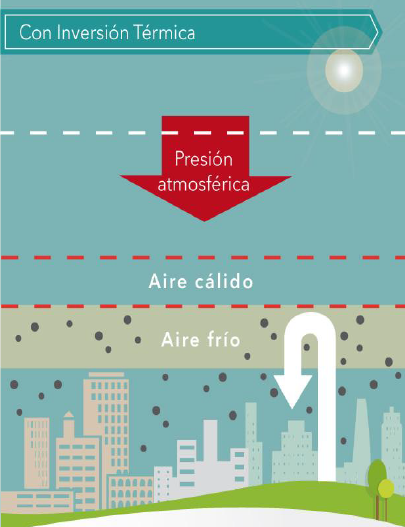
\includegraphics[scale=0.5]{Imagenes/Inversion_Termica_02.png}
\end{figure}
\end{frame}
\begin{frame}
\frametitle{Definición de la inv. térmica}
Debido a que se presenta una estabilidad del aire impidiendo cualquier tipo de intercambio vertical quedando atrapados los contaminantes.
\end{frame}
\begin{frame}
\frametitle{Definición de la inv. térmica}
Arriba de la capa de aire caliente existe otra capa de aire frío a una mayor altura.
\end{frame}

\end{document}